
\chapter{Process Development and Integration of Power MEMS Devices}
\label{ch:Process Development and Integration of Power MEMS Devices}

% **************************** Define Graphics Path **************************
\ifpdf
    \graphicspath{{Chapter7/Figs/Raster/}{Chapter7/Figs/PDF/}{Chapter6/Figs/}}
\else
    \graphicspath{{Chapter7/Figs/Vector/}{Chapter7/Figs/}}
\fi


In this chapter, I would develop the corresponding fabrication process parameters and their process integration based on the manufacturing technology and equipment in Chapter Three, thus realizing the whole process \index{Fabrication process} from GaN wafer to device. In order to simplify the expression of the process and clarify the steps of the process, this chapter uses different codes to represent the different steps and their meanings. For example MESA.3) indicates that this process is the third step in the mesa preparation process, and [AE-N] indicates the alignment and exposure of negative photoresist. The process that first appears in this chapter would be described in detail about the main purpose of the process, the equipment used, and the detailed recipe parameters and shorthand code, while the same process in the following steps is only represented by the shorthand code. I've listed every step without omission based on shorthand code. Moreover, in order to visualize the fabrication process flow, a corresponding flow chart has been drawn to illustrate the main process steps.

\section{Process flow and recipe}

\begin{figure}[H] 
\centering    
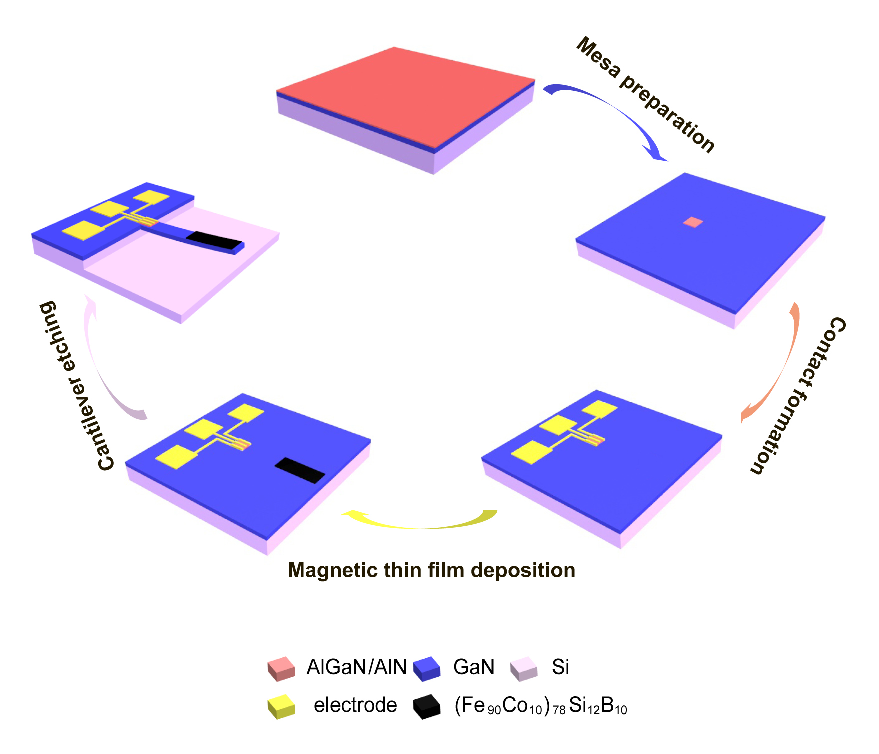
\includegraphics[width=0.8\textwidth]{processflow}
\caption[The schematic diagram of process flow]{The schematic diagram of process flow}
\label{fig:processflow}
\end{figure}

The fabrication process flow chart of GaN power MEMS is shown in the \autoref{fig:processflow}, which can be roughly divided into four main steps. The first step is mesa isolation, and the device is isolated by ICP etching. The second step is to deposit the source, drain and gate metal electrodes to realize the HEMT device. The third step is the deposition of the magnetic thin film at the front end of the cantilever (there is no such step for the SPD device). The fourth step is to etch the cantilever structure. The realization of each step is inseparable from the pattern transfer of photomask, so \autoref{fig:layout} shows the layout (drawn with AutoCAD) during the fabrication. The specific steps will be described in detail in the subsections.

\begin{figure}[H] 
\centering    
\includegraphics[width=0.9\textwidth]{mask}
\caption[Layout of GaN power MEMS devices]{Layout \index{Photomask} of GaN power MEMS devices}
\label{fig:layout}
\end{figure}


\subsection{Wafer growth}

\begin{figure}[H] 
\centering    

\includegraphics[width=0.7\textwidth]{structure}
\caption[GaN-on-SiC wafer hetero-epitaxial structure]{GaN-on-SiC wafer hetero-epitaxial structure}
\label{fig:structure}
\end{figure}


The \index{Fabrication process} epitaxial growth \index{Epitaxial!growth} of GaN wafer \index{Wafer} is a fundamental step in the research of group III nitride semiconductors. Due to the difficulty in obtaining large-scale and high-quality GaN bulk substrates, GaN epitaxial layers are still mainly grown on foreign substrates. The most widely used are sapphire, SiC, and Si. which have a large lattice mismatch \index{Lattice!mismatch} with GaN. To address this problem, Amano et al. developed a two-step growth method in 1986. The AlN nucleation layer is first grown at low temperature, and then raised to high temperature to grow GaN layer, which greatly improves the quality of the GaN epitaxial layer \cite{amano1986metalorganic}. In 1989, Akasaki et al. systematically studied and improved the two-step method, first using low temperature to deposit AlN or GaN as a buffer layer, and then desired GaN material is grown on the buffer layer in a high temperature environment \cite{akasaki1989effects}.

The \index{Fabrication process} hetero-expitaxial structure of 3-inch GaN-on-Si wafer is shown in \autoref{fig:structure}. From bottom to top are 1 \unit{mm} Si(111) substrate, 3.5 $\sim$ 4 \unit{\um} AlN/AlGaN multi-layer buffer layer, 400 $\sim$ 600 \unit{\nm} unintentionally doped (UID) GaN buffer layer, 300 \unit{\nm} intrinsic GaN 2DEG channel layer, 1 \unit{\nm} AlN barrier layer, 20 \unit{\nm} AlGaN barrier layer and 2 \unit{\nm} GaN cap layer. The lattice mismatch between the Si substrate and the GaN 2DEG channel layer is alleviated by different Al composition of the AlN/AlGaN buffer layer, and the lattice mismatch between the AlN/AlGaN layer and the GaN 2DEG \index{Two-dimensional electron gas (2DEG)} channel \index{Channel} layer is further adjusted by the UID GaN buffer layer. The grown wafer exhibits good electrical performance with 300 \unit{\ohm}/square  sheet resistance, \num{1.00e13} \unit{\per\square\cm} carrier \index{Carrier!concentration} density, 2000 \unit{cm^2/(Vs)} mobility \index{Electron mobility} and \SI{600}{\volt} breakdown \index{Voltage!breakdown voltage} voltage.

\subsection{Pre-processing}
During \index{Fabrication process} pre-processing, the dice \index{Dice} of size \numproduct{2 x 2} \unit{mm} and \numproduct{3 x 3} \unit{mm} firstly have been cut from the grown 3-inch wafers with the DISCO DAD3350 automatic dicing saw. Because there are a lot of particles and organic contaminants on the surface \index{Surface} of the cut dice, the dice would be then strictly cleaned by cleaning technologies. The recipe is listed here:

\begin{description}
	\item[PRE.1)] Wafer \index{Dice} dicing [WD].
	\item[PRE.2)] A complete RCA cleaning \index{Cleaning!RCA cleaning} process ($\times$ 1 time) [WET-RCA].
	\item[PRE.3)] Piranha solution \index{Piranha solution} with the \ce{H2SO4} (98$\%$) and \ce{H2O2} (30$\%$) in 7:3 ratios, sonicated for 10 minutes ($\times$ 1 time) [WET-PA].
	\item[PRE.4)] Sonicate in acetone solution for 5 minutes ($\times$ 3 times) [WET-ACE].
	\item[PRE.5)] Sonicate in \index{Cleaning!wet cleaning} ethanol solution for 5 minutes ($\times$ 3 times) [WET-ETH].
	\item[PRE.6)] Sonicate in deionized water \index{Deionized water} for 5 minutes ($\times$ 3 times) [WET-DIW].
	\item[PRE.7)] Sonicate in hydrochloric acid \index{Hydrochloric acid} for 5 minutes ($\times$ 3 times) [WET-HC].
	\item[PRE.8)] [WET-DIW]
	\item[PRE.9)] Nitrogen gas drying [GD-N].
	\item[PRE.10)] Dry cleaning \index{Cleaning!dry cleaning} in PVA TePla IoN 40 plasma cleaner with 80 sccm Oxygen gas and \SI{100}{\watt} power for 1 min ($\times$ 1 time) [DC-OX].
\end{description}


\subsection{Mesa preparation}

In \index{Fabrication process} order \index{Photoresist} to isolate different devices on a single die, mesa \index{Mesa isolation} isolation, often referred to as active area \index{Active region} isolation, is required. We first transfer the active area pattern from photomask \index{Photomask} to \index{Dice} dice by \index{Photolithography} photolithography, and then etch the mesa by ICP-RIE. The size of the active area \index{Active region} is \numproduct{34 x 34} \unit{um^2}, and the photomask is prepared as shown in the \autoref{fig:active area}, where the cross pattern marks are mainly used for subsequent overlay alignment. The main steps are as follows:

\begin{description}

	\item[MESA.1)] Photoresist coating
	
	Spin coating SUN-9i \index{Photoresist} negative photoresist produced by Suntific Material (Weifang), Ltd. The rotation speed is 500 rpm/min for the first 8 seconds and 5000 rpm/min for the last 40 seconds [PC-N].
	
	\item[MESA.2)] Post-apply bake
	
	After \index{Fabrication process} coating, the resulting resist film will contain between 20$\%$ $\sim$ 40$\%$ by weight solvent. The post-apply bake \index{Post-apply bake} process, also called a soft-bake or a pre-bake, involves drying the photoresist after spin coating by removing this excess solvent. The main reason for reducing the solvent content is to stabilize the photoresist film \cite{mack2008fundamental}. In this process, the post-apply baking recipe is \SI{110}{\degreeCelsius} for 60 seconds [PAB-N].
	
	\item[MESA.3)] Alignment and exposure
	
\begin{figure}[H] 
\centering    
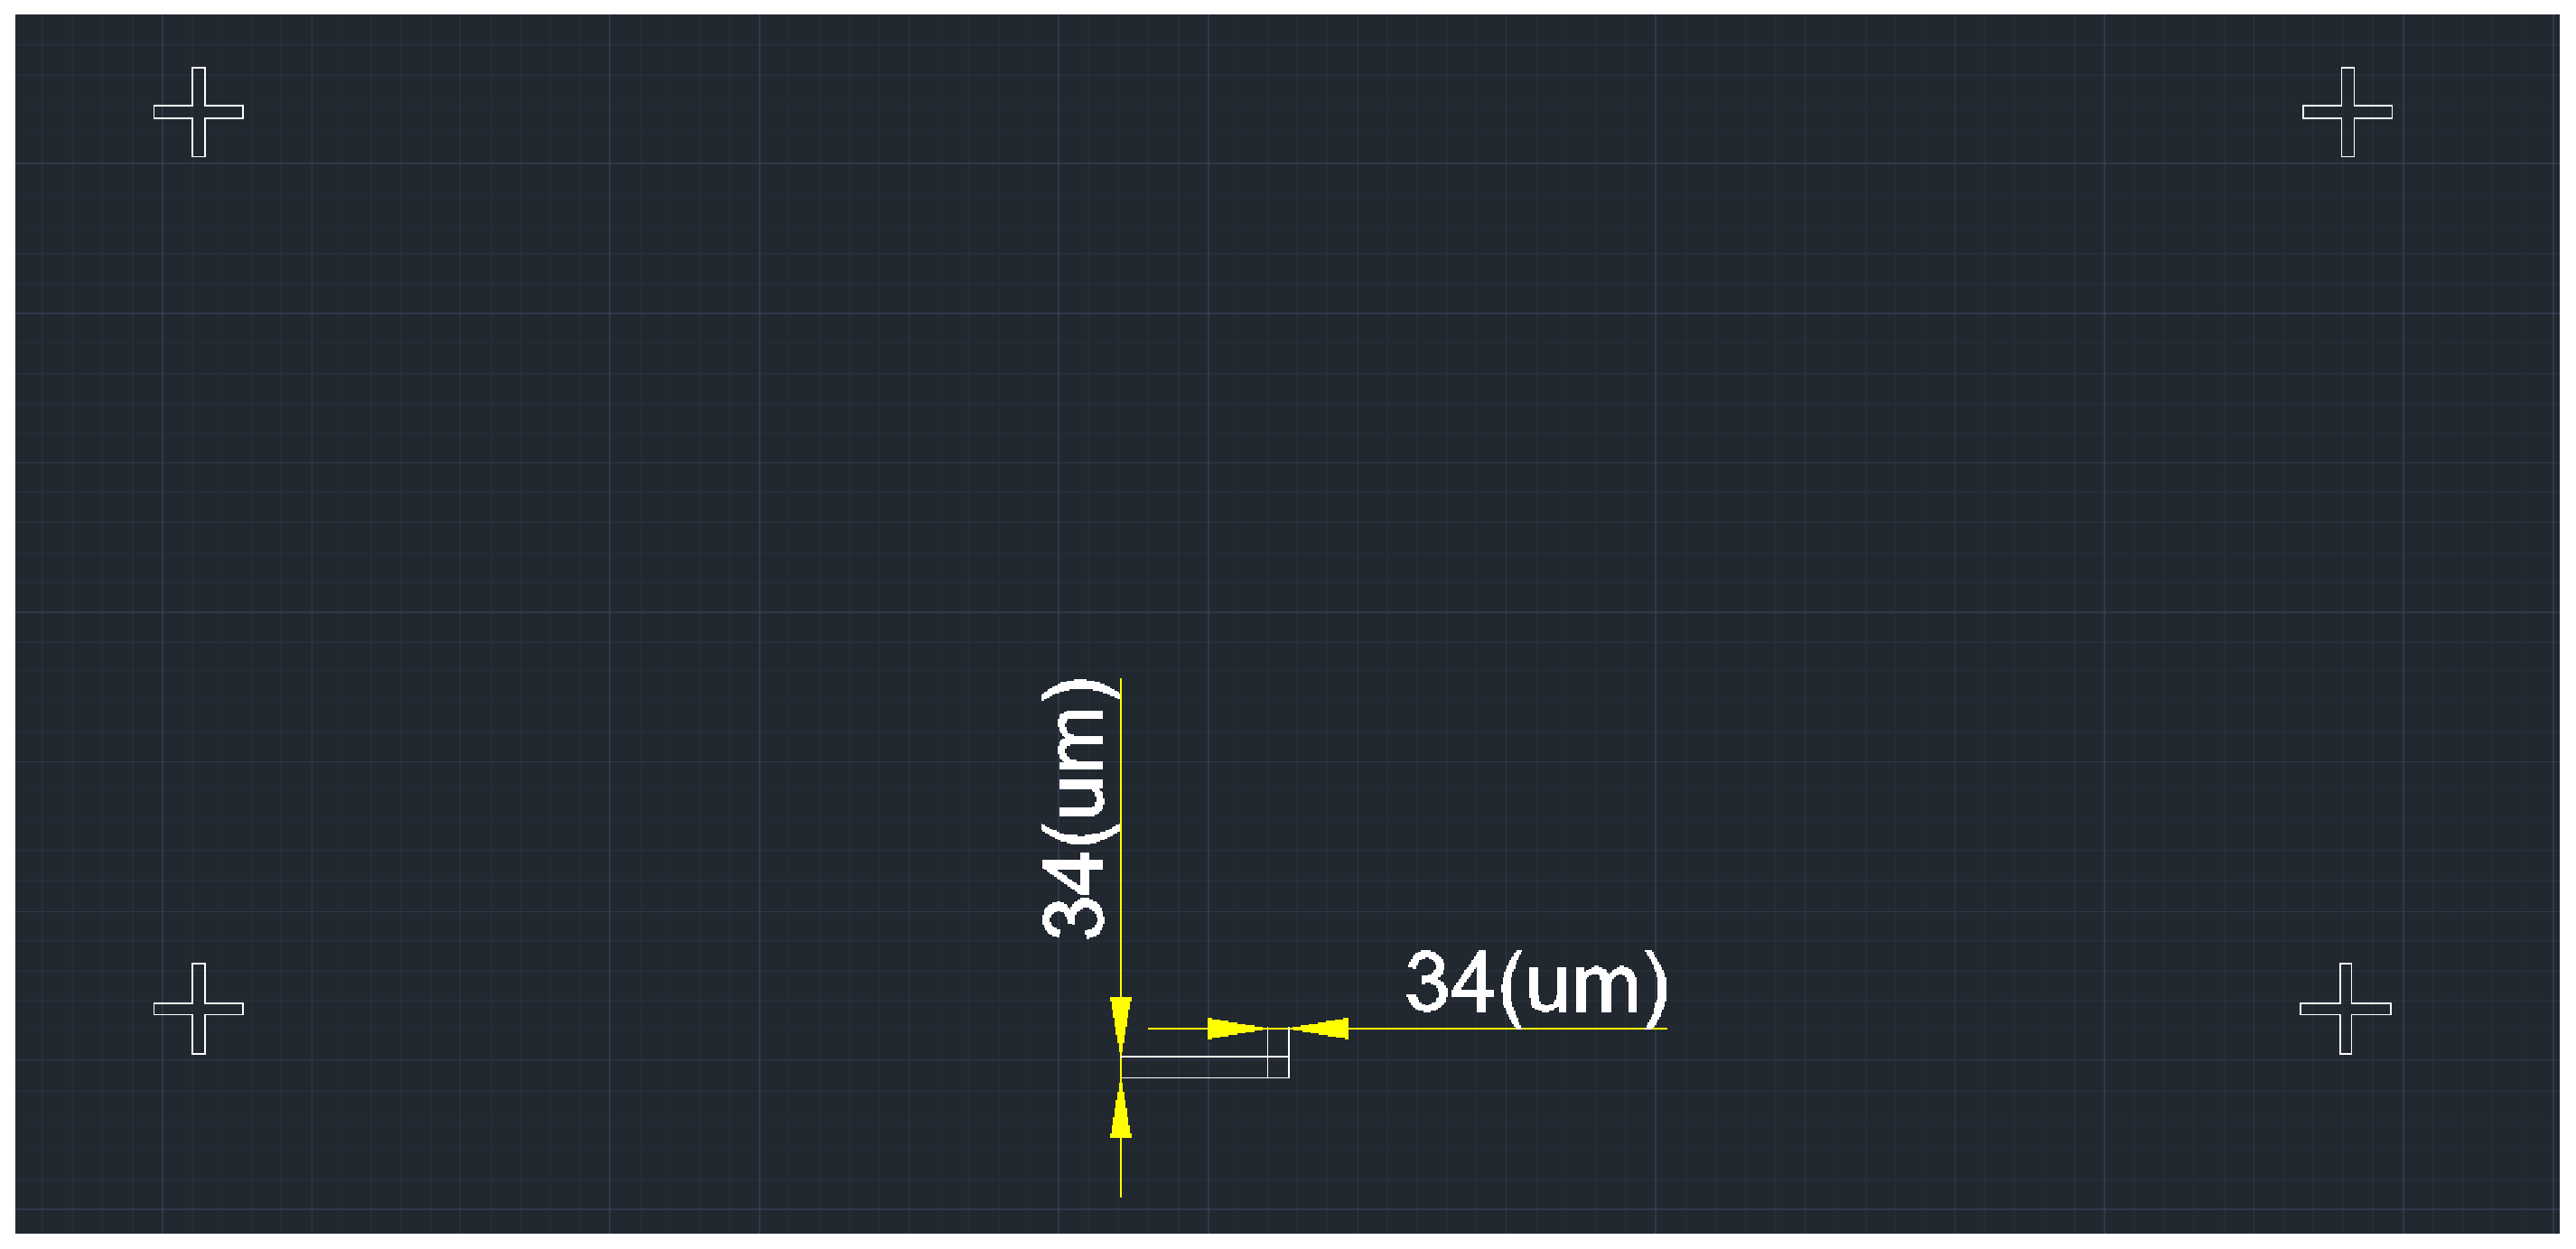
\includegraphics[width=0.9\textwidth]{active area}
\caption[Photomask of active area]{Photomask \index{Photomask} of active area}
\label{fig:active area}
\end{figure}
	
	Align and exposure with SUSS MA6 mask aligner, and exposure parameters are as follows: Process: Lithography, Exposure time: 30 seconds, Alignment gap: 50 \unit{um}, Contact type: Soft, WEC type: Cont, WEC-offset: OFF [AE-N].
	
	\item[MESA.4)] Post-exposure bake
	
	Post-exposure bake \index{Post-exposure bake} is one method of reducing the standing wave effect \cite{mack2008fundamental}. The recipe is \SI{140}{\degreeCelsius} for 60 seconds [PEB-N].
	
	\item[MESA.5)] Development
	
	Once \index{Photoresist} exposed, the photoresist \index{Photoresist} must be developed. The aqueous and tetramethyl ammonium hydroxide (TMAH) are commonly used as developers. Development is undoubtedly one of the most critical steps in the photoresist process. The characteristics of the resist-developer interactions determine to a large extent the shape of the photoresist profile and, more importantly, the linewidth control \cite{mack2008fundamental}. The development recipe is to first stir and soak in developer solution \index{Developer solution} SUN-238D produced by Suntific Material (Weifang), Ltd for 40 seconds, and then stir and soak in \index{Deionized water} deionized water for 20 seconds [DEV-N].	
	
	\item[MESA.6)] [GD-N]
	
	\item[MESA.7)] [DC-OX]
	
	\item[MESA.8)] ICP-RIE etching
	 
	 In \index{Fabrication process} order \index{Photoresist} to isolate the \index{Mesa isolation} mesa, all epitaxial layers above the AlN/AlGaN multi-layer buffer layer except the active area \index{Active region} must be removed, including UID GaN buffer layer, intrinsic GaN 2DEG \index{Two-dimensional electron gas (2DEG)} channel \index{Channel} layer, AlN barrier layer, AlGaN barrier layer and GaN cap layer. The total etching thickness is about 1000 \unit{\nm}. The etching process has been performed with SENTECH SI 500 ICP-RIE \index{Inductively coupled plasma (ICP)} and the etching recipe is as follows: Etching gas: \ce{BCl3}/\ce{Cl2}/\ce{O2} (10/32/5 sccm), Etching power: \SI{550}{\watt}, RF power: \SI{100}{\watt}. The etching rate is 200 \unit{nm/min}, and the total etching time is 10 minutes [DE-MESA].
	 
	\item[MESA.9)] [WET-ACE]
	
	\item[MESA.10)] [WET-ETH]
	
	\item[MESA.11)] [WET-DIW]
	
	\item[MESA.12)] [GD-N]
	
	\item[MESA.12)] [DC-OX]
		
\end{description}


\subsection{Metal-semiconductors contact formation}

After \index{Fabrication process} the isolation \index{Mesa isolation} of the \index{Active region} active region, the next step begins to prepare the gate Schottky contact \index{Contact!Schottky contact} and the source-drain \index{Contact!Ohmic contact} ohmic contact. The source-drain ohmic contact would been prepared first, with an area of \numproduct{6 x 34} \unit{um^2}. By depositing Ti, Al, Ni, Au metals in sequence and undergoing rapid thermal \index{Rapid thermal!annealing (RTA)} annealing, a good ohmic contact has been formed on the GaN \index{Surface} surface. The Schottky contacts are then further formed by depositing Ni and Au, with an area of \numproduct{5 x 34} \unit{um^2}. The prepared gate contact has good control performance on electrons in the channel. For the convenience of subsequent electrical tests, the photomask \index{Photomask} of the contact also includes a pad with a much larger area (about \numproduct{1000 x 1000} \unit{um^2}).

\begin{description}

	\item[CTC.1)] [PC-N]
	\item[CTC.2)] [PAB-N]
	\item[CTC.3)] [AE-N]
	
\begin{figure}[H] 
\centering    
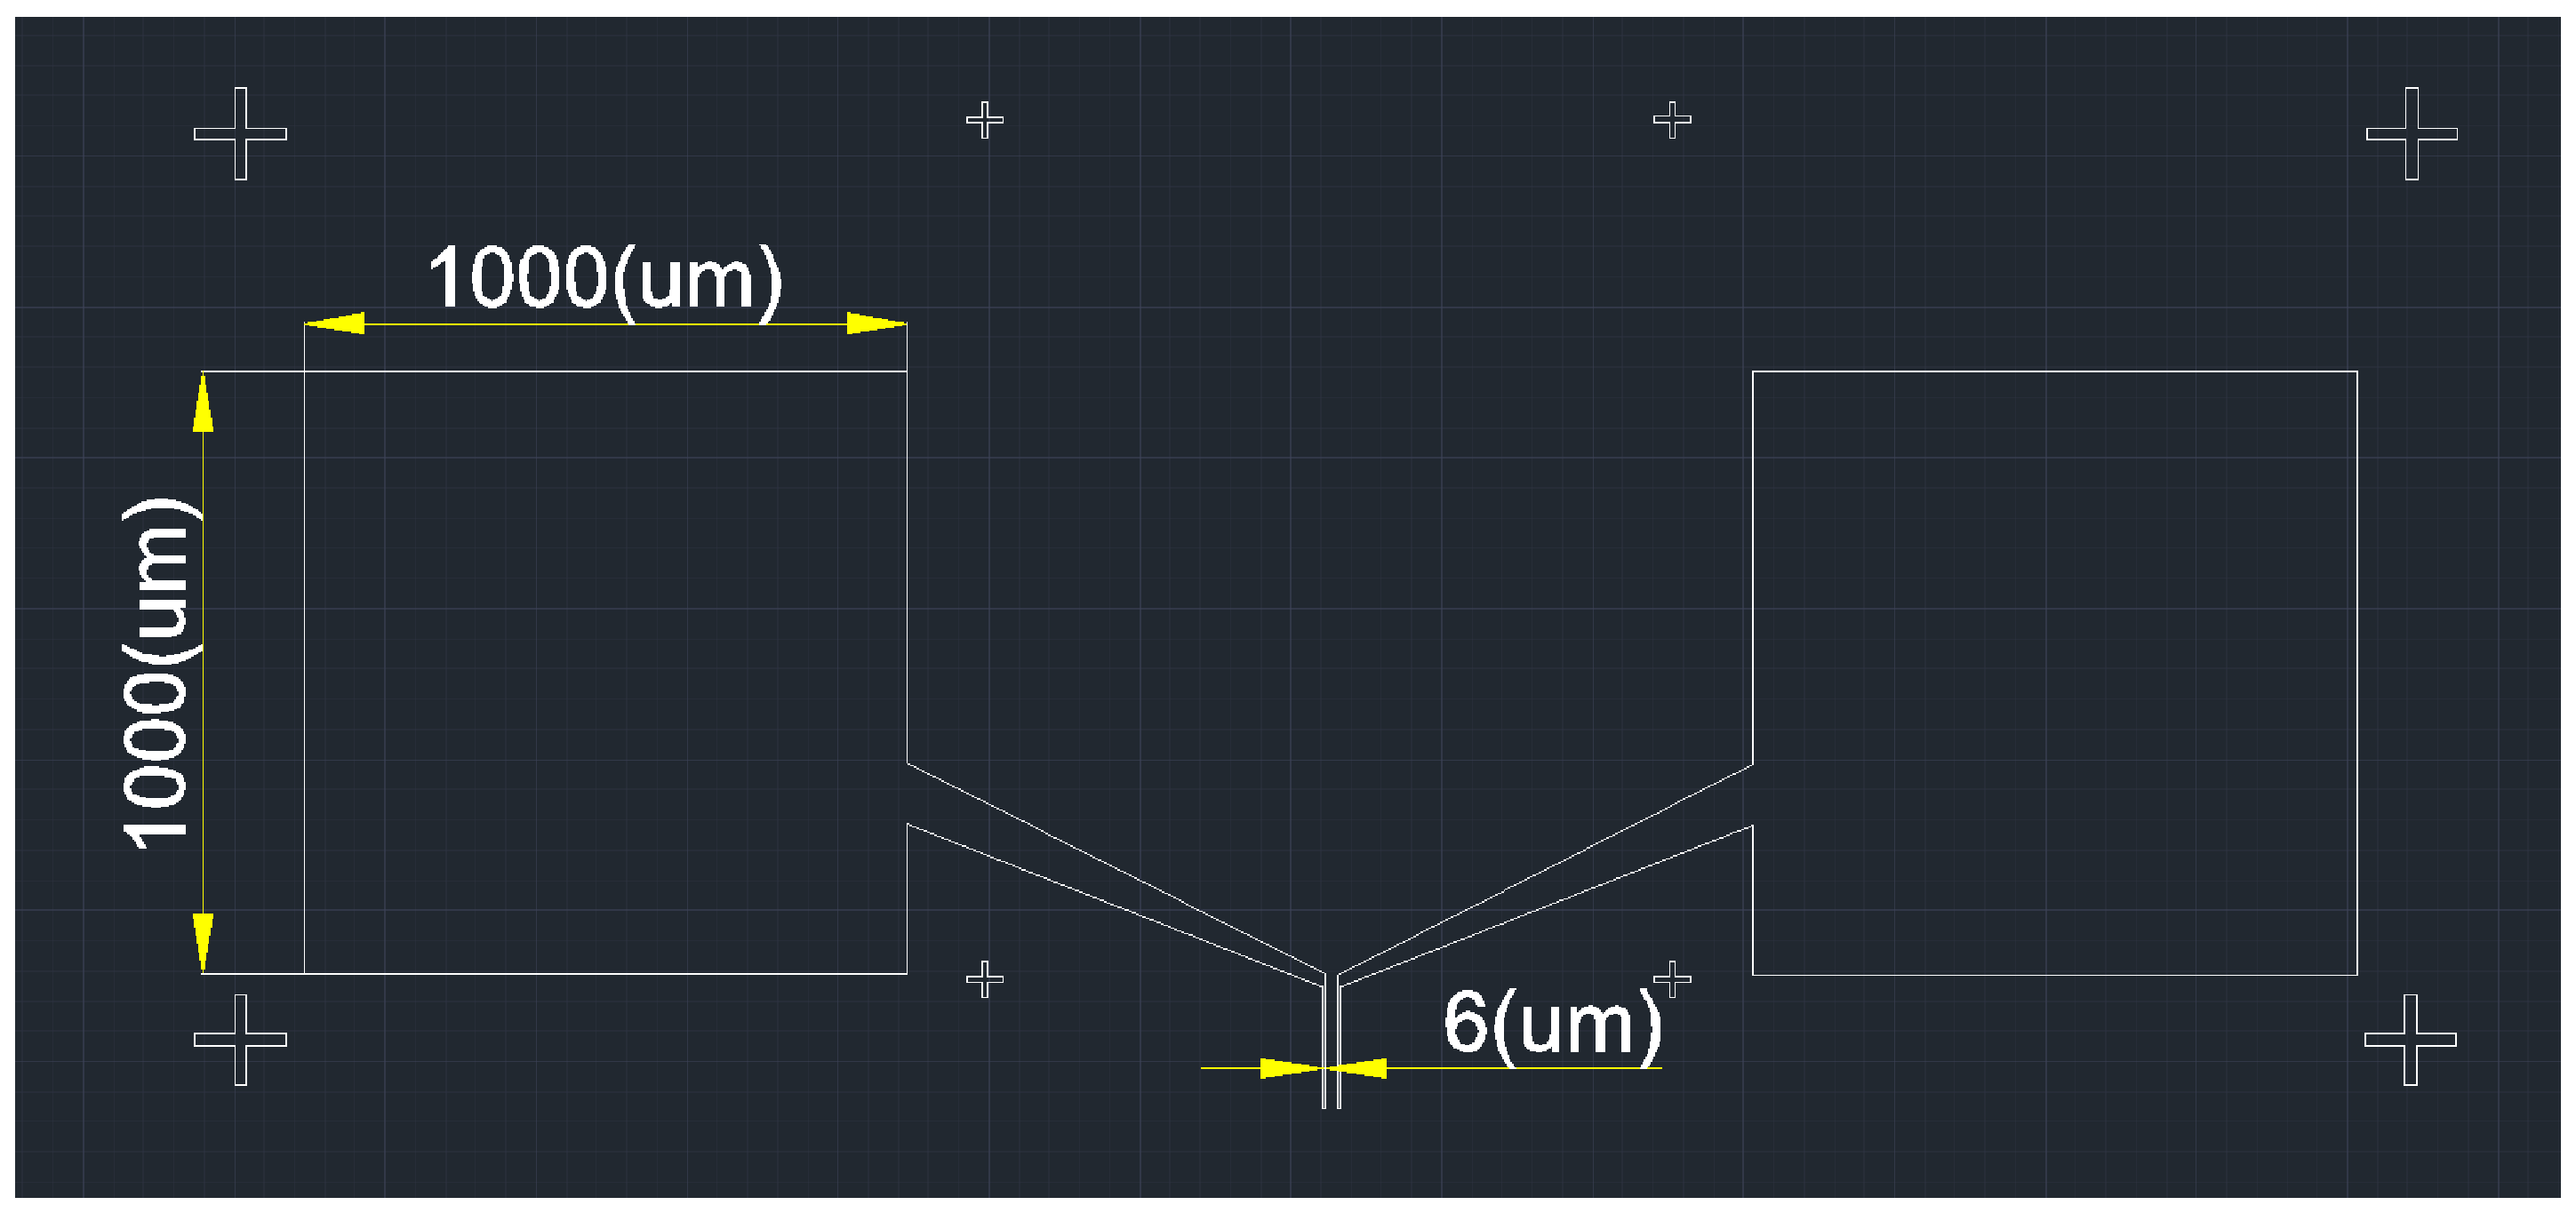
\includegraphics[width=0.9\textwidth]{source}
\caption[Photomask of source and drain contact]{Photomask \index{Photomask} of source and drain contact}
\label{fig:source}
\end{figure}

	\item[CTC.4)] [PEB-N]
	
	\item[CTC.5)] [DEV-N]
	
	\item[CTC.6)] [GD-N]
	
	\item[CTC.7)] [DC-OX]
	
	\item[CTC.8)] Source-drain metal deposition
	
	The \index{Fabrication process} source-drain \index{Photoresist} contact metal is Ti, Al, Ni, Au. Ti is a barrier metal and must have a work function (3.95 \unit{\eV}) that approximates the affinity potential of GaN (4.11 \unit{\eV}), and therefore is the most widely used barrier metal. Al is a commonly used capping layer, its work function is 4.25 \unit{\eV}, and it can also promote the solid-phase chemical reaction between N atoms and the barrier metal Ti. Ni acts as a diffusion barrier metal, preventing the interdiffusion of the cap layer metal Au and the barrier layer metal Al to the surface \index{Surface} of the GaN material. Au is a stable, low-resistance noble metal ideal for use as a cap layer metal.
	
	In this research, from the bottom (GaN surface) to the top, Ti with a thickness of 20 \unit{\nm}, Al with a thickness of 120 \unit{\nm}, Ni with a thickness of 45 \unit{\nm}, and Au with a thickness of 55 \unit{\nm} have been deposited using Denton Vacuum Explore 14 E-beam evaporation system at deposition rates of \SI{0.5}{\angstrom}/s, \SI{1}{\angstrom}/s, \SI{0.5}{\angstrom}/s and \SI{0.5}{\angstrom}/s, respectively [DEP-SD].
	
	\item[CTC.9)] [WET-ACE]
	
	\item[CTC.10)] [WET-ETH]
	
	\item[CTC.11)] [WET-DIW]
	
	\item[CTC.12)] [GD-N]
	
	\item[CTC.13)] [DC-OX]
	
	\item[CTC.14)] Rapid thermal processing
	
	Rapid \index{Fabrication process} thermal \index{Rapid thermal!processing (RTP)} processing (RTP) \index{Rapid thermal!annealing (RTA)} of the deposited Ti, Al, Ni, Au metal is necessary in order to form an \index{Contact!Ohmic contact} ohmic contact. In this work, rapid thermal annealing at \SI{850}{\degreeCelsius} for 30 seconds has been performed using a LABSYS RTP-1200 rapid thermal processing system [RTP-OHM].
	
	\item[CTC.15)] [WET-ACE]
	
	\item[CTC.16)] [WET-ETH]
	
	\item[CTC.17)] [WET-DIW]
	
	\item[CTC.18)] [GD-N]
	
	\item[CTC.19)] [DC-OX]
	
	\item[CTC.20)] [PC-N]
	\item[CTC.21)] [PAB-N]
	\item[CTC.22)] [AE-N]
	
\begin{figure}[H] 
\centering    
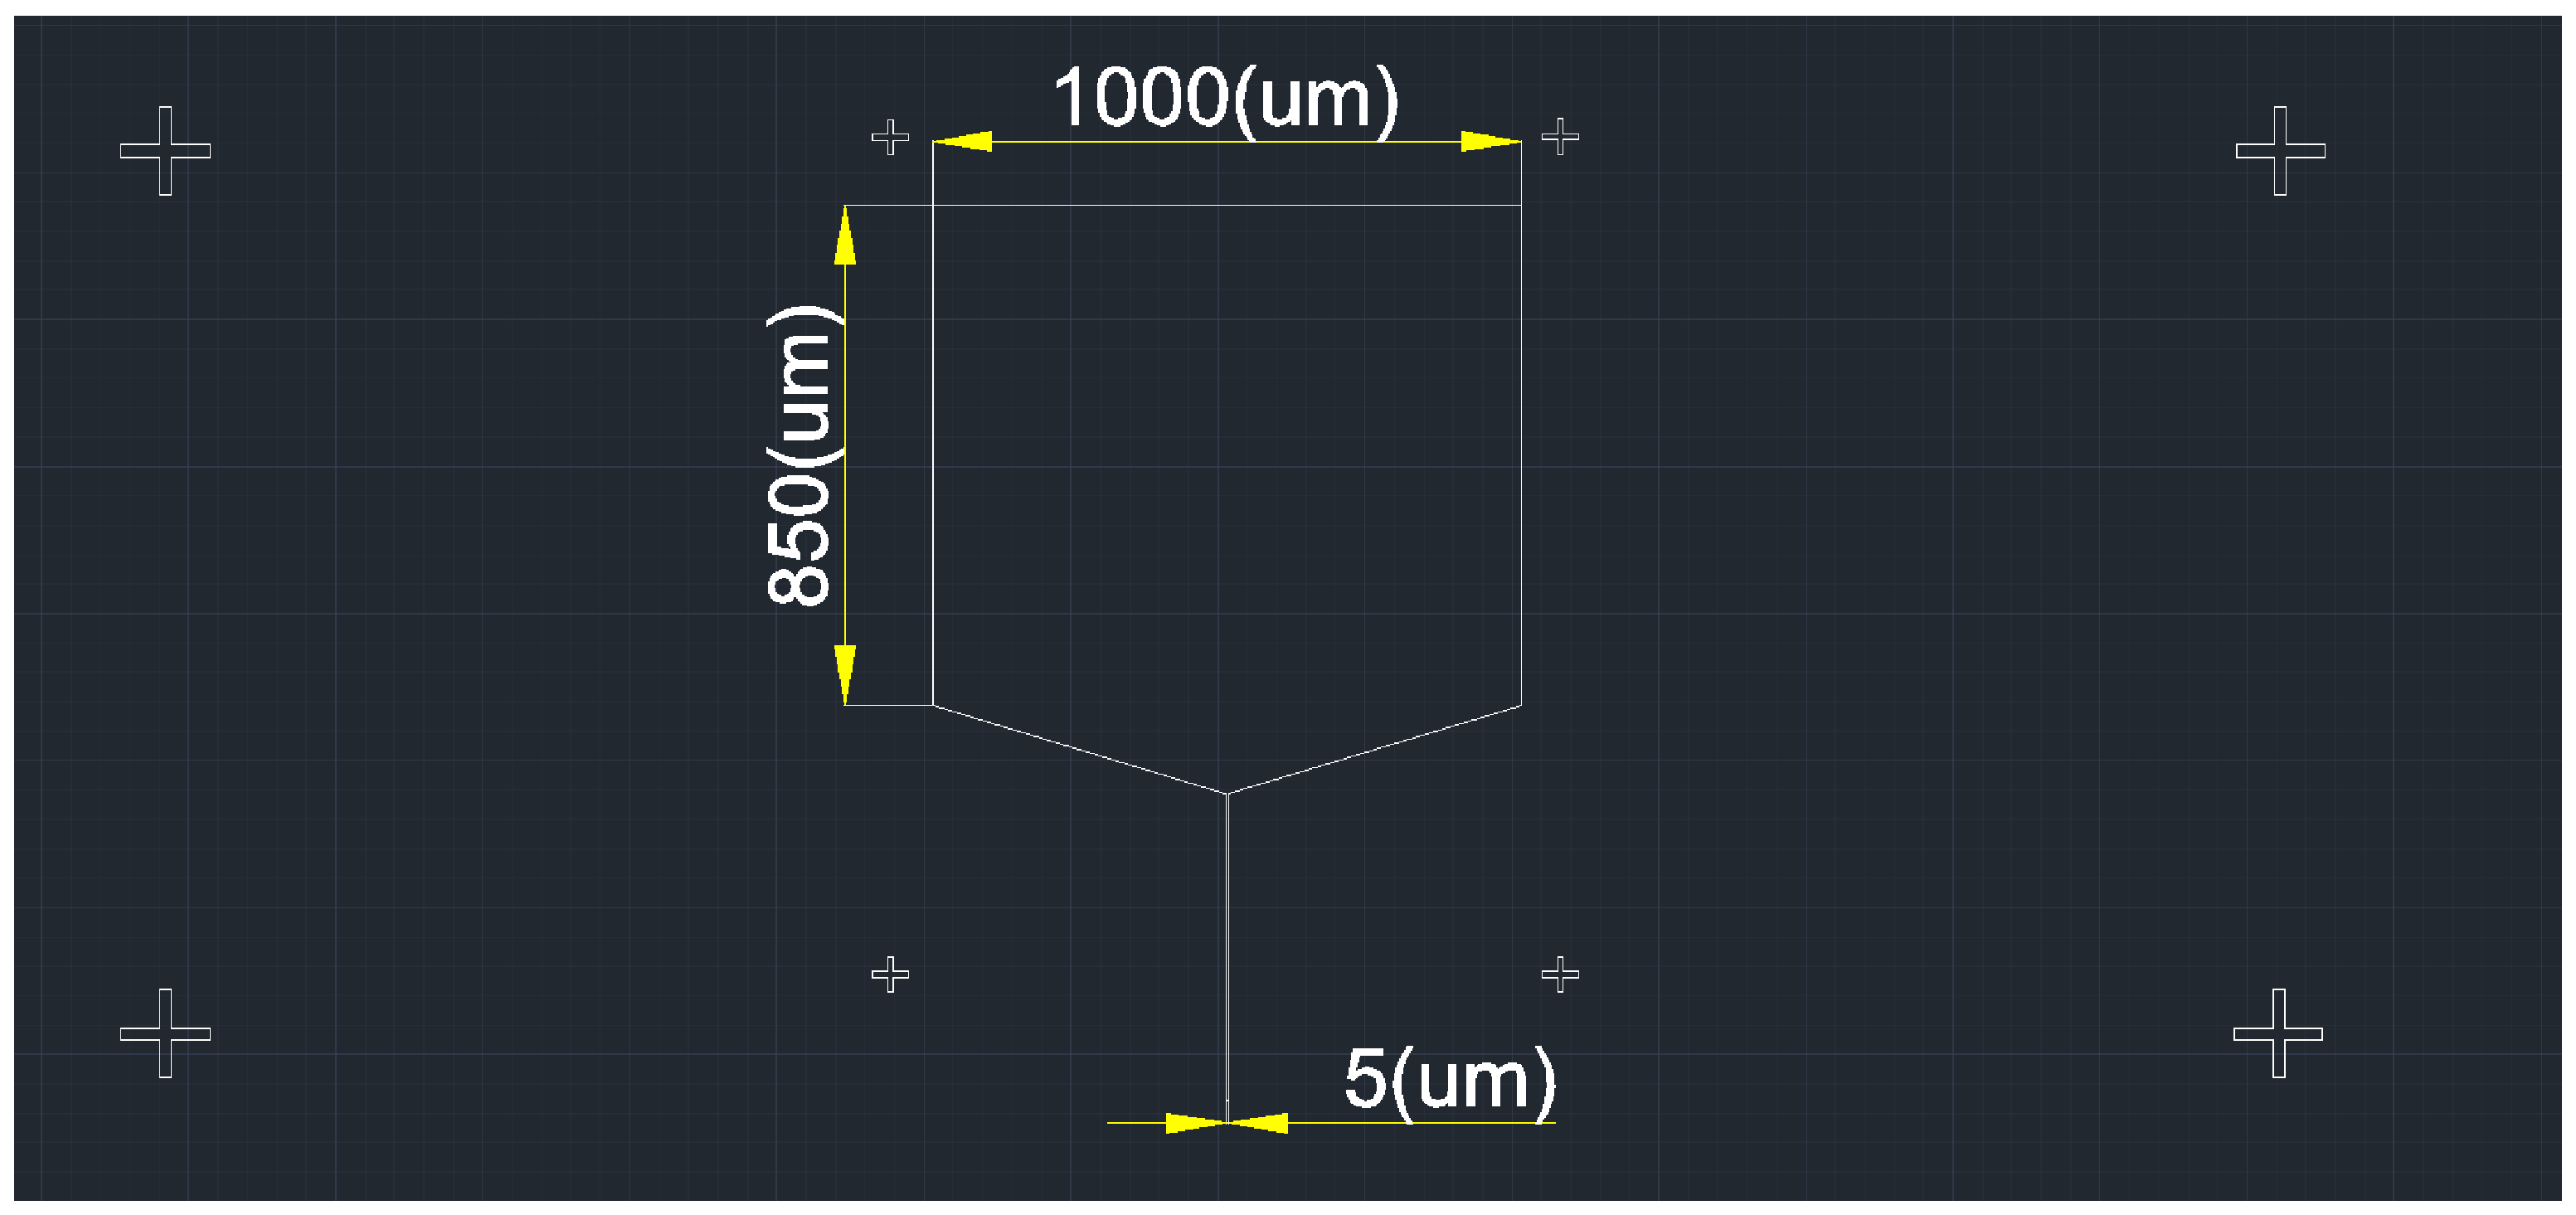
\includegraphics[width=0.9\textwidth]{gate}
\caption[Photomask of gate contact]{Photomask \index{Photomask} of gate contact}
\label{fig:gate}
\end{figure}
	
	\item[CTC.23)] [PEB-N]
	
	\item[CTC.24)] [DEV-N]
	
	\item[CTC.25)] [GD-N]
	
	\item[CTC.26)] [DC-OX]
	
	\item[CTC.27)] Gate metal deposition

	The \index{Photoresist} gate \index{Contact!Schottky contact} contact metal is Ni, Au from the bottom (GaN surface) to the top. Ni with a thickness of 80 \unit{\nm}, and Au with a thickness of 50 \unit{\nm} have been successively deposited using Denton Vacuum Explore 14 E-beam evaporation system at deposition rates of \SI{0.5}{\angstrom}/s and \SI{0.5}{\angstrom}/s, respectively [DEP-G].
		
	\item[CTC.28)] [WET-ACE]
	
	\item[CTC.29)] [WET-ETH]
	
	\item[CTC.30)] [WET-DIW]
	
	\item[CTC.31)] [GD-N]
	
	\item[CTC.32)] [DC-OX]
	
\end{description}

Until \index{Fabrication process} now, I have prepared an AlGaN/AlN/GaN \index{HEMT} HEMT device on \index{Wafer} GaN-on-Si wafer. The active region \index{Active region} is \numproduct{34 x 34} \unit{um^2}, the gate is a Ti/Au Schottky contact with a width of 5 \unit{um}, and the source and drain are Ti/Al/Ni/Au ohmic \index{Contact!Ohmic contact} contact with a width of 6 \unit{um}. The electrical characteristics of HEMT are shown in the \autoref{fig:performancehemt}. It can be seen from the figure that HEMT exhibits good Schottky contacts \index{Contact!Schottky contact} on the gate and ohmic contacts on the source and drain (\autoref{fig:performancehemt}c,d). Based on the good electrical contact performance, the output characteristics ($I_{ds}-V_{ds}$) of HEMT have excellent gate control capabilities, as shown in \autoref{fig:performancehemt}a. Therefore, the output current \index{Output!current} exhibits good linearity at low source-drain bias ($V_{ds}$) voltage, and then as the bias voltage further increases, the output current reaches saturation. HEMT can achieve stable large current output in the saturation region, and can be effectively controlled at various \index{Voltage!gate voltage} gate voltage $V_{gs}$ from \SI{-7}{\volt} to \SI{1}{\volt}. The maximum current density at \SI{1}{\volt} gate voltage reaches 304 \unit{\mA\per\mm}, and the maximum transconductance \index{Transconductance} reaches 42.4 \unit{\milli\siemens\per\mm}, showing excellent electrical performance. Moreover, the gate leakage current \index{Current!leakage current} and source-drain leakage current of HEMT are also within a \index{Fabrication process} reasonable range (\autoref{fig:performancehemt}e,f).

\begin{figure}[H] 
\centering    
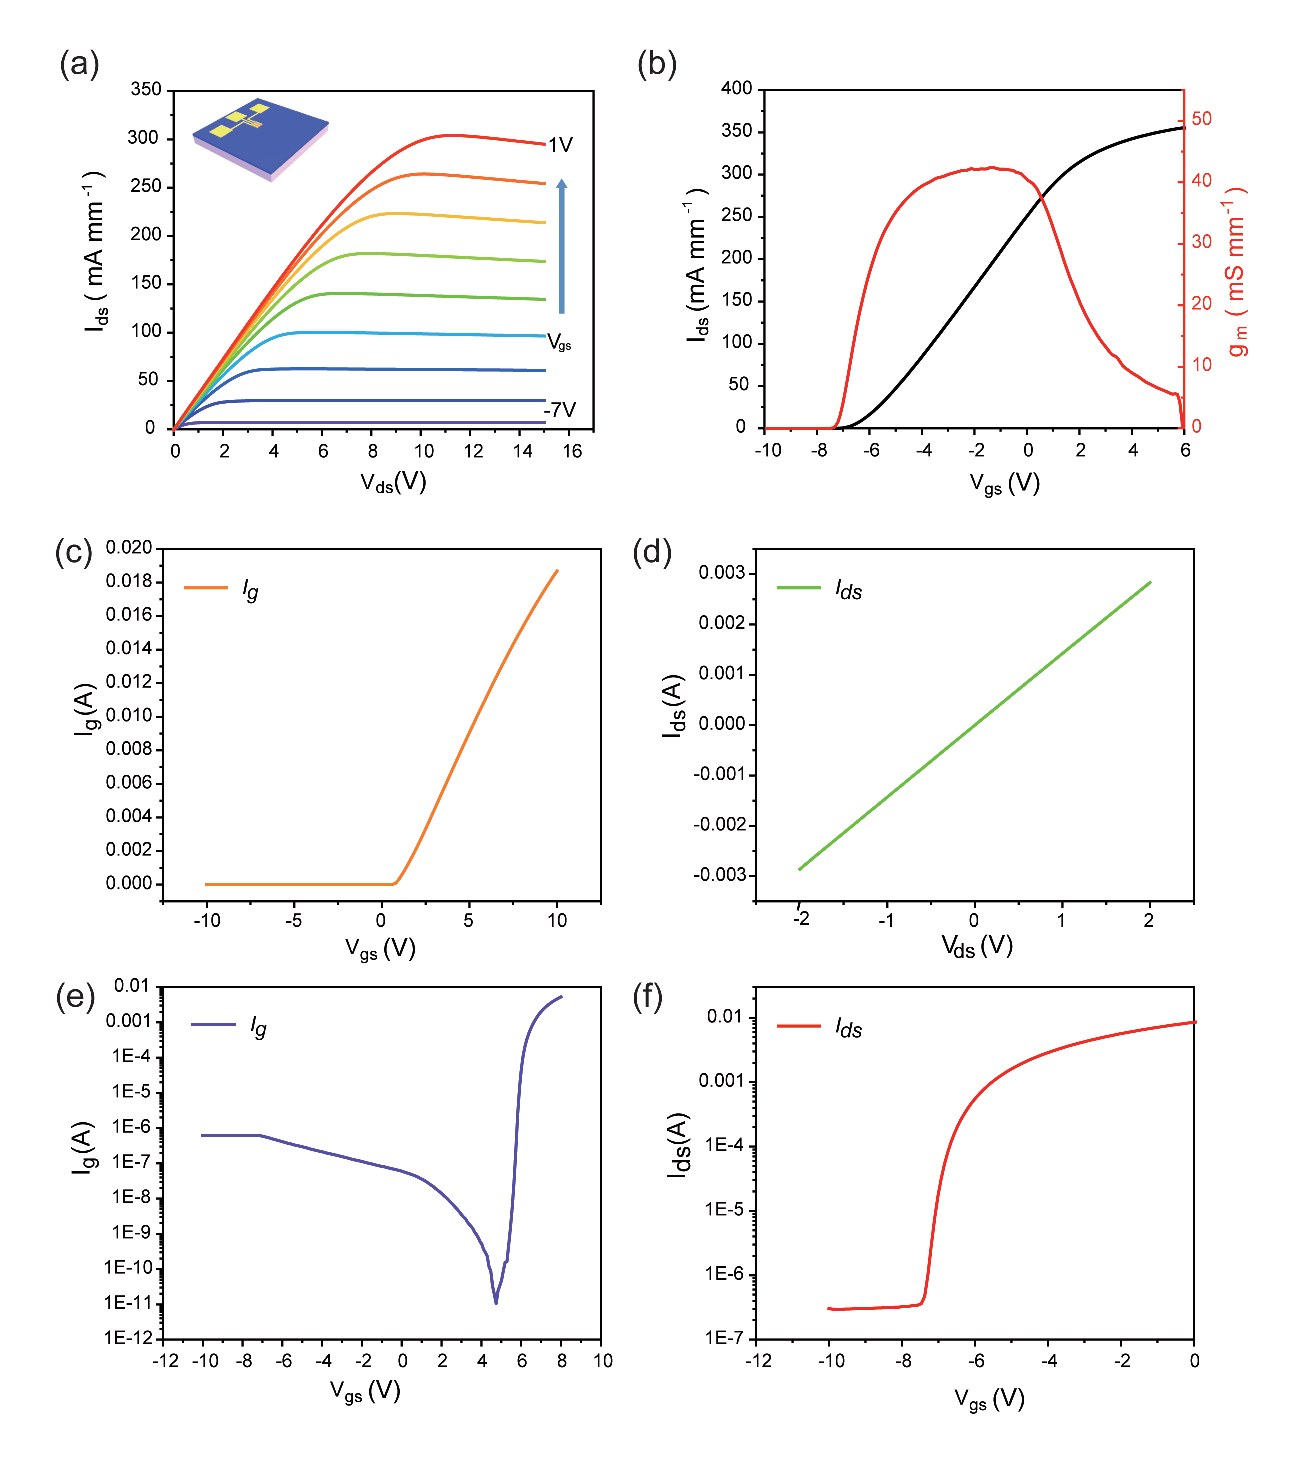
\includegraphics[width=0.9\textwidth]{performancehemt}
\caption[Electrical performance of fabricated AlGaN/AlN/GaN HEMTs]{Electrical performance of fabricated AlGaN/AlN/GaN HEMTs}
\label{fig:performancehemt}
\end{figure}



\subsection{Magnetic thin film deposition (For MPD)}

Before \index{Fabrication process} the \index{Photoresist} preparation of cantilever, there is one more process which is unique to \index{Magnetosensory power MEMS devices (MPD)} MPD. This process aims to deposit a magnetic \index{Magnetic!thin film} thin film \index{Thin film} on the top half \index{Cantilever} of the cantilever, which can generate magnetic forces in different directions at the front of the cantilever under the action of external \index{Magnetic!field} magnetic field. The size of the mask is \numproduct{175 x 60} \unit{um^2}, and it is located in the front half of the cantilever, where the size of the cantilever is \numproduct{350 x 60} \unit{um^2}. 

\begin{description}
	\item[MAG.1)] [PC-N]
	\item[MAG.2)] [PAB-N]
	\item[MAG.3)] [AE-N]

\begin{figure}[H] 
\centering    
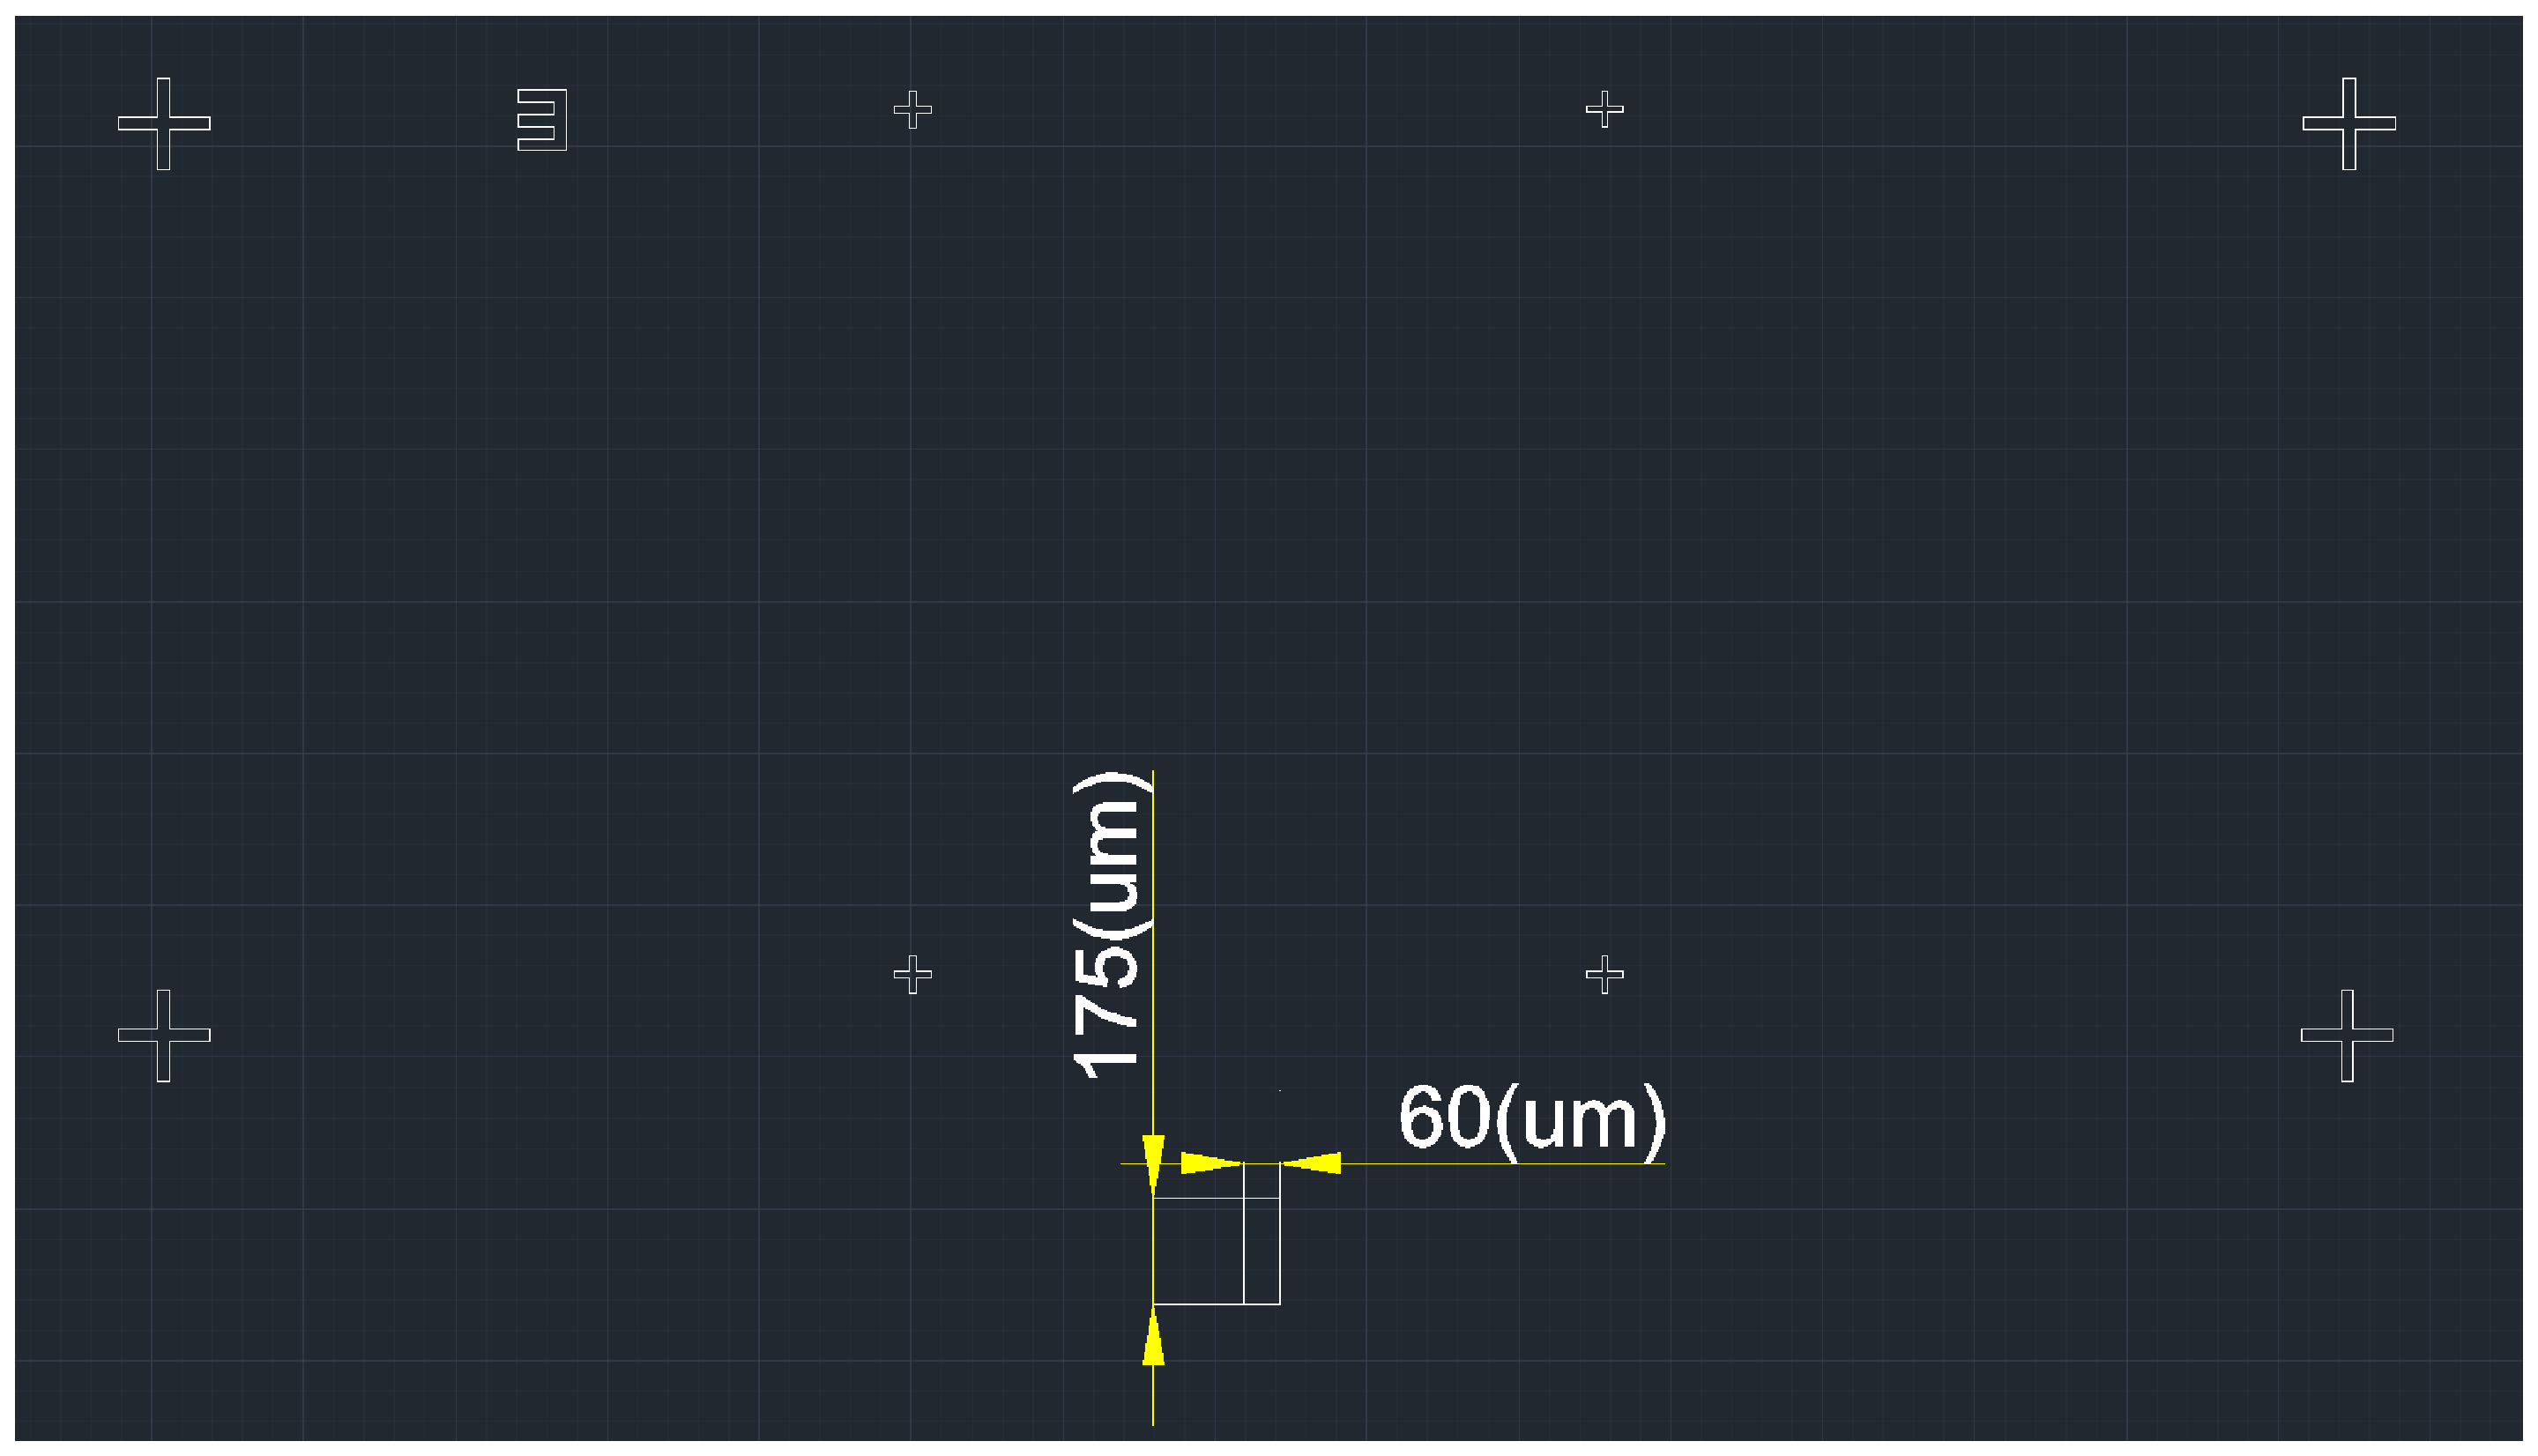
\includegraphics[width=0.9\textwidth]{magnetic film}
\caption[Photomask of magnetic film]{Photomask \index{Photomask} of magnetic film}
\label{fig:magnetic film}
\end{figure}

	\item[MAG.4)] [PEB-N]
	
	\item[MAG.5)] [DEV-N]
	
	\item[MAG.6)] [GD-N]
	
	\item[MAG.7)] [DC-OX]
	
	\item[MAG.8] Magnetic thin film deposition
	
	The \index{Photoresist} Denton Discovery 635 magnetron sputtering \index{Deposition!magnetron sputtering} system has been applied to deposit 500 \unit{\nm} thick \index{Magnetic!thin film} magnetic thin film \ce{(Fe90Co10)78Si12B10}. The recipe is as follow: DC sputtering, Gas: Ar 135 sccm, Power: \SI{400}{\watt}, Pressure: 7.2 mtorr. The deposition rate is 15 \unit{nm/min}, and the deposition time is 33.3 min [DEP-MAG].
	
	\item[MAG.9)] [WET-ACE]
	
	\item[MAG.10)] [WET-ETH]
	
	\item[MAG.11)] [WET-DIW]
	
	\item[MAG.12)] [GD-N]
	
	\item[MAG.13)] [DC-OX]
	

\end{description}

\subsection{GaN cantilever preparation}

Finally, the \index{Fabrication process} ICP-based \index{Inductively coupled plasma (ICP)} dry \index{Photoresist} etching has been performed by combing the \index{Etching!isotropic etching} anisotropic/isotropic etching \index{Etching!anisotropic etching} to fabricate the \index{Cantilever} cantilever. The main steps of the etching process are as follows: Step 1: anisotropic etching of photoresist patterned GaN (thickness: 5 \unit{\um}). Step 2: isotropic etching of Si to release the cantilever. The manufactured cantilever has dimensions of \numproduct{350 x 60 x 5} \unit{um^3}. For the final fabricated \index{MEMS} MEMS devices, the SPD has only a single cantilever, while the MPD has a cantilever with a magnetic thin film in the front half end.
	
\begin{description}

	\item[CAN.1)] Photoresist coating
	
	Spin coating AZ4620 positive photoresist produced by Suntific Material (Weifang), Ltd. The rotation speed is 500 rpm/min for the first 8 seconds and 3500 rpm/min for the last 60 seconds [PC-P].
	
	\item[CAN.2)] Post-apply bake
	
	The pre-baking \index{Post-apply bake} recipe is \SI{95}{\degreeCelsius} for 3 minutes [PAB-P].
	
	\item[CAN.3)] [PC-P]
	

	\item[CAN.4)] [PAB-P]
	
	
	\item[CAN.5)] Alignment and exposure
	
\begin{figure}[H] 
\centering    
\includegraphics[width=0.9\textwidth]{cantilever}
\caption[Photomask of GaN cantilever]{Photomask of GaN cantilever}
\label{fig:cantilever}
\end{figure}

	Align \index{Cantilever} and exposure \index{Photomask} with SUSS MA6 mask aligner, and exposure parameters are as follows: Process: Lithography, Exposure time: 54 seconds, Alignment gap: 30 \unit{\um}, Contact type: Soft, WEC type: Cont, WEC-offset: OFF [AE-P].

	\item[CAN.6)] Development
	
	The \index{Fabrication process} developing \index{Photoresist} recipe is firstly immersed in a 3:1 solvent of deionized \index{Deionized water} water \index{Developer solution} and developer solution AZ-400K produced by Santaifu Materials (Weifang), Ltd, and then stirred and immersed in deionized water. The time needs to be determined in real time according to the real-time observation of the optical microscope (about 4 $\sim$ 5 \unit{\minute}) [DEV-P].
	
	\item[CAN.7)] [GD-N]
	
	\item[CAN.8)] [DC-OX]
	
	\item[CAN.9)] ICP-RIE etching

	 To \index{Fabrication process} fabricate the \index{Cantilever} cantilever, an anisotropic etching \index{Etching!anisotropic etching} must first be performed to etch the GaN, AlN and AlGaN layers, and then an isotropic \index{Etching!isotropic etching} etching of Si must be performed to release the cantilever. The etching process is performed with SENTECH SI 500 ICP-RIE. Firstly, the GaN etching recipe is as follows: Etching gas: \ce{BCl3}/\ce{Cl2}/\ce{Ar} (10/32/5 sccm), Etching power: \SI{550}{\watt}, RF power: \SI{100}{\watt}. The etching rate is 200 \unit{nm/min}, and the total etching time is 25 min. Secondly, the Si etching recipe is as follows: Etching gas: \ce{SF6}/\ce{O2}/\ce{Ar} (30/5/10 sccm), Etching power: \SI{800}{\watt}, RF power: \SI{50}{\watt}. The lateral etching rate is 2 \unit{um/min}, and the total etching time is 25 min [DE-CAN].
	 
	 \item[CAN.10)] [DC-OX]	

\end{description}

In this section, I have successfully prepared the GaN power \index{MEMS} MEMS devices with cantilever \index{Cantilever} structure. The electrical characteristics of MPD are shown in the \autoref{fig:performancempd}. MPD \index{Magnetosensory power MEMS devices (MPD)} exhibits electrical properties similar to \index{HEMT} HEMT. However, compared with HEMT, the current of MPD under the bias voltage of \SI{10}{\volt} is reduced by 60.5 \unit{\mA\per\mm}. The gate leakage current \index{Current!leakage current} and source-drain leakage current of MPD are also slightly larger than HEMT, as shown in \autoref{fig:performancempd}e,f. Furthermore, the transfer ($I_{ds}-V_{gs}$) characteristics of the MPD at $V_{ds}$ = \SI{10}{\volt} has also been measured. The maximum transconductance \index{Transconductance} ($g_{m, max}$) of MPD is 32.9 \unit{\milli\siemens\per\mm} (\autoref{fig:performancempd}b), while the value for the HEMT can reach 42.4 \unit{\milli\siemens\per\mm} (\autoref{fig:performancehemt}b). Therefore, the transconductance performance of MPD is also slightly lower than HEMT due to the performance degradation \index{Degradation} caused by dry etching process. 

It can be concluded that, compared with the HEMT device before etching, the performance of the MPD device is reduced by about 30$\%$. This is because the long-term ICP \index{Inductively coupled plasma (ICP)} etching weakens the contact performance of the \index{Electrode} electrode, and the removal of the Si \index{Substrate} substrate releases the lattice strain \index{Lattice!strain} of AlGaN/AlN/GaN \index{AlGaN/AlN/GaN heterojunction} heterojunction. This is also because the dry etching \index{Etching!dry etching} process has caused damage to the lattice structure of the material. The performance degradation \index{Degradation} of MEMS devices before and after etching is discussed in detail in the \index{Cantilever} next \index{Fabrication process} subsection.

\begin{figure}[H] 
\centering    
\includegraphics[width=0.9\textwidth]{performancempd}
\caption[Electrical performance of fabricated MPD]{Electrical performance of fabricated \index{Magnetosensory power MEMS devices (MPD)} MPD}
\label{fig:performancempd}
\end{figure}

\section{Mechanisms of process-induced performance degradation}

This \index{Fabrication process} section briefly discusses the physical mechanisms \index{Physical!mechanism} of MEMS device performance degradation \index{Degradation} before and after the ICP-RIE \index{Inductively coupled plasma (ICP)} etching process. By means of Raman spectroscopy \index{Raman!spectroscopy} and literature review, the effects of lattice strain \index{Lattice!strain} release and introduction of lattice defects \index{Lattice!defects} during the cantilever \index{Cantilever} fabrication process on device performance have been revealed respectively.

\subsection{Lattice strain relief and piezoelectric effect}

\begin{figure}[H] 
\centering    
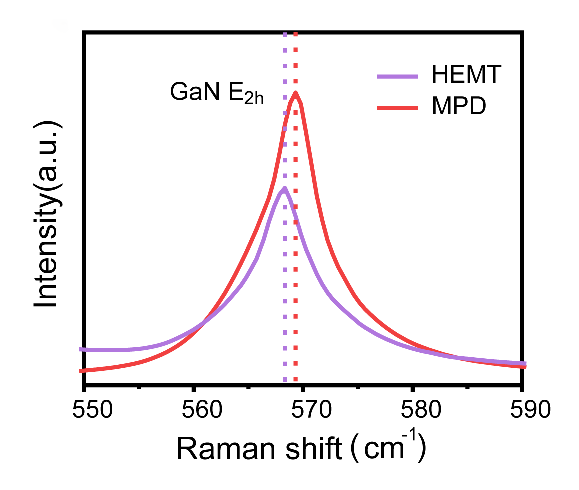
\includegraphics[width=0.7\textwidth]{ramanmpd}
\caption[Raman spectroscopy of fabricated HEMT and MPD]{Raman spectroscopy of fabricated HEMT and MPD}
\label{fig:ramanmpd}
\end{figure}

In order to reveal the physical mechanism \index{Physical!mechanism} of process-induced performance loss, the Raman spectroscopy tests on both HEMT \index{HEMT} and MPD \index{Magnetosensory power MEMS devices (MPD)} at room temperature have been performed to explain the influence of the ICP dry etching \index{Etching!dry etching} process on the electrical performance of MEMS, as shown in \autoref{fig:ramanmpd}. It exhibits that the $E_{2h}$ phonon mode of MPD shows a blue shift from 568.31 \unit{\per\cm} to 569.33 \unit{\per\cm} compared with the HEMT, which reveals that the dry etching process releases the silicon substrate and relaxes the tensile strain of the GaN layer \cite{yang2015influence,wang2016piezotronic}. The relationship between the biaxial stress \index{Biaxial stress model} and the shift of the Raman phonon frequency is shown in \autoref{eq:raman} 
\begin{equation}
\sigma _{a}=\frac{\Delta \omega}{K_{\mathrm{RS}}^{\mathrm{E} 2(h i g h)}}
\label{eq:raman}
\end{equation}
where $\sigma _{a}$ is the \index{In-plane biaxial stress} in-plane biaxial stress, $\Delta \omega$ is the shift of the Raman \index{Raman!phonon frequency} phonon frequency, and $K_{\mathrm{RS}}^{\mathrm{E} 2(h i g h)}$ is the Raman biaxial stress conversion \index{Raman!biaxial stress conversion factor} factor. We can obtain that the tensile strain of the GaN epitaxial layer \index{Epitaxial!layer} is reduced by 352 \unit{\MPa} compared with that on the Si \index{Substrate} substrate \cite{choi2013analysis}. According to the \index{Piezoelectric!effect} piezoelectric effect, the removal of the Si substrate partially releases the lattice \index{Lattice!strain} strain of the GaN layer, thereby changing the piezoelectric polarization charge \index{Piezoelectric!polarization charge} of the GaN layer, adjusting the energy band \index{Energy band} of the heterostructure, and finally reducing the density of 2DEG \index{Two-dimensional electron gas (2DEG)} in the \index{AlGaN/AlN/GaN heterojunction} AlGaN/AlN/GaN heterojunction.

\subsection{Lattice defects and Schottky contact degradation}

In \index{Fabrication process} addition, a large number of lattice defects \index{Lattice!defects} have also been introduced during the \index{Etching!dry etching} dry etching process, which reduces the electrical performance of MPD \index{Magnetosensory power MEMS devices (MPD)} to a certain extent \cite{ladroue2010deep,pearton2000review,huang2004inductively}. Moreover, it has been reported that the \index{Inductively coupled plasma (ICP)} ICP etching could introduce lattice defects and surface state to the AlGaN/AlN/GaN heterojunction \index{AlGaN/AlN/GaN heterojunction} and massive damage to contact \index{Electrode} electrode, which will form electron trap levels. This will result in the increase of ideality factor and the leakage current, thereby significantly reducing the gate control ability \cite{cao2000schottky,choi2003observation,fang2003etching,JieLiu2007Influence}. Last but not least, the etching of the Si substrate under the cantilever will also greatly weaken the heat dissipation in the active area. All these effects enhance the self-heating effect \index{Self-heating effect} of the \index{MEMS} MEMS device, thus impairing the \index{Output!current} output current performance \cite{yang2011high,hajjiah2020effect,greco2017temperature}.

In summary, ICP \index{Inductively coupled plasma (ICP)} dry etching could inevitably degrade \index{Degradation} the performance of \index{MEMS} MEMS during the preparation of the \index{Cantilever} cantilever. Comparing the performance of \index{Magnetosensory power MEMS devices (MPD)} MPD and \index{HEMT} HEMT, it can be concluded that due to the ICP etching process in the cantilever fabrication process, the electrical performance of MPD has been degraded to a certain extent compared to HEMT devices. It has shown that this performance degradation \index{Degradation} is unavoidable in the process of fabricating cantilever \index{Cantilever} structures using the ICP process, but we have improved the performance degradation during cantilever \index{Cantilever} fabrication through process optimization. Compared to the electrical performance of SPD \index{Strain-controlled power MEMS devices (SPD)} in \autoref{ch:Strain-controlled power devices}, the electrical performance of \index{Magnetosensory power MEMS devices (MPD)} MPD in \autoref{ch:Magnetosensory Power Devices} has been greatly improved, which is detailed in the process optimization \index{Inductively coupled plasma (ICP)} subsection.

\section{Process optimization}

Since \index{Fabrication process} the successful preparation of SPD, the huge performance loss of SPD before and after etching has been the biggest process problem. How to significantly improve the performance of MEMS devices in the preparation of MPD has become the primary issue. After persistent experiments and analysis, I finally succeeded in finding a process optimization method that greatly improves the performance of MEMS devices. The core idea is how to protect the active area \index{Active region} and \index{Electrode} electrode contacts of \index{MEMS} MEMS during long-time cantilever \index{Cantilever} ICP-RIE etching. Therefore, starting with photoresist coating and ICP-RIE etching, two complementary optimized processes have been developed.

\subsection{Positive photoresist double coating process}

In this process, we need to choose a suitable photoresist \index{Photoresist} as the etching mask for the cantilever \index{Cantilever} and increase the withstanding time during the ICP etching. Because the ICP etching time of cantilever is so long that the ordinary photoresist mask can not withstand, here I choose AZ4620 positive photoresist produced by Suntific Material (Weifang), Ltd. Moreover, photoresist needs to be thick or hard enough to be used as an etching mask. There could be two main methods here. One method is to spin coat the photoresist twice to increase the thickness of the photoresist, and the other one is to harden the photoresist in some ways. I choose the first method here, and maybe explore the second method in the future. The first spin coating velocity is 3500 rpm/min, and the coating time is one minute. After post-apply bake \index{Post-apply bake} for 3 minutes at \SI{95}{\degreeCelsius}, the thickness of photoresist is about 9 \unit{\um}. Then spin coat at 3500 rpm/min for another one minute and bake for 3 minutes at \SI{95}{\degreeCelsius} again. The total thickness of photoresist is about 18 \unit{\um} now, and is thick enough to withstand long-time ICP etching.

\subsection{GaN cantilever ICP-RIE etching process}

In \index{Fabrication process} this process, how to maximize the withstanding time of photoresist during the \index{Inductively coupled plasma (ICP)} ICP etching process is the most important issue. Since plasma etching will generate extremely high heat which will greatly reduce the hardness of the photoresist, it is necessary to apply silicone oil to the bottom of the wafer \index{Wafer} before etching to enhance heat dissipation. Furthermore, it is significant to carefully control the chamber temperature. Through the alternate etching steps of short-time etching and long-time cooling, the temperature in the chamber is maintained at no more than \SI{10}{\degreeCelsius}. 

The etching condition of the cantilever \index{Cantilever} can be judged by optical microscope and \index{Scanning electron microscopy (SEM)} SEM, and the judgment method of optical microscope is more convenient and has been introduced here. Because the band gap of GaN, AlN, and AlGaN is larger than the energy of visible light, AlGaN, AlN, and GaN are all transparent and we can directly observe the Si substrate \index{Substrate} through an optical microscope. When etching Si isotropically, we can observe the real-time situation of lateral etching of Si under the GaN cantilever, and judge the etching process of the cantilever \index{Cantilever} in real time.

These optimized processes have successfully realized cantilever structure MEMS devices with excellent electrical performance, which has become the most important process in the fabrication of GaN power MEMS devices.

\section{Summary}

In this chapter, I use the processing equipment described in \autoref{ch:Manufacturing Technology of Power MEMS Devices} to introduce the fabrication process and process flow of GaN power MEMS \index{MEMS} devices in detail. There are six main parts in the preparation process, and a total of about eighty specific steps. The purpose, recipe, and precautions of each process are briefly described. The description of repetitive processes is simplified by means of process integration, and therefore the logical structure of the fabrication process is highlighted. More importantly, the physical mechanism and process optimization of performance degradation during MEMS device fabrication are analyzed. As a result, high-performance GaN HEMTs and GaN power MEMS devices have been successfully \index{Fabrication process} fabricated.



